\documentclass[twocolumn,a4paper,10pt,review,5p]{elsarticle}

\usepackage{amsmath}
\usepackage{lineno,hyperref}
\usepackage{tabularx}
\usepackage{amssymb}
\usepackage{booktabs}
\modulolinenumbers[5]

\journal{Journal of Web Semantics}

%% `Elsevier LaTeX' style
\bibliographystyle{elsarticle-num}

%%%%%%%%%%%%%%%%%%%%%%%

\begin{document}

% =========================================
% front matter

\begin{frontmatter}

\title{Adversarial Ranking for Knowledge Graph Representation with Ensemble}

% ----------------------
% affiliations

\author[hrbaddress]{Qingsong Meng}

\author[ucasaddress,hrbaddress]{Xiang Zhang}
\ead{xiang.zhang@nlpr.ia.ac.cn} % `ead' stands for email address

\author[ucasaddress]{Shizhu He}
\ead{shizhu.he@nlpr.ia.ac.cn}

\author[ucasaddress]{Jun Zhao\corref{correspondingauthor}}
\ead{jzhao@nlpr.ia.ac.cn}

\cortext[correspondingauthor]{Corresponding author}
\address[hrbaddress]{Harbin University of Science and Technology, No.52 Xuefu Road, Nangang District, Harbin, 150080, China}
\address[ucasaddress]{University of Chinese Academy of Sciences, No.19(A) Yuquan Road, Shijingshan District, Beijing, P.R.China 100049}

% -------------------------
% abstract + keywords

\begin{abstract}
Adversarially training.
\end{abstract}

\begin{keyword}
Knowledge Graph \sep{} Representation Learning \sep{} Adversarial Training \sep{} Ensembel Learning
\MSC[2010] 68T30 \sep{} 68T50
\end{keyword}

\end{frontmatter}

% ==========================================
% main text

\linenumbers{}

% ------------------------
% introduction

\section{Introduction}
\label{sec:intro}

Knowledge graph is an important component in many natural language processing applications nowadays, such as natural language inference, question answering, and task-oriented dialogue generation. One of the fundamental tasks in the field is \emph{representation learning}, which aims to learn a representation for each \emph{entity} and \emph{relation} in a knowledge graph. Consider the following example. The triple \emph{(Leonhard Euler, BornIn, Basel)} is a selected fact from a typical knowledge graph, \emph{WikiData}\footnote{https://www.wikidata.org/}. Representation learning models assign a vectorized representation respectively to the head entity \emph{Leonhard Euler} and the tail entity \emph{Basel}, and some models also give a representation for each relation, namely \emph{BornIn} in this example. In general, there must be some characteristics to hold or constraints to meet for these representations, which facilitate other tasks like inference or completion on the knowledge graph.

% TODO: avoid using formula but to use graphs instead in introduction

One of the most popular constraints is the translation assumption. Borders et al.~\cite{TransE2013} first proposed the \emph{TransE} model, in which the representation of a tail entity~$(t)$ could be arithmetically computed by adding the representations of the corresponding head entity~$(h)$ and relation~$(r)$, that is, $h + r \simeq t$. This gives a very concise and beautiful geometric explanation that every relation can move or \emph{translate} an entity embedding into another, and hence its name \emph{TransE}.
The model is trained by minimize a hinge loss with a predefined margin between the scores of positive and negative samples. The score in TransE is given by an L1 or L2 norm or the vector $h + r - t$, which can be seen as a special scoring (or energy) function.

These models can be seen as \textbf{discriminative models} that share the same framework but differ in the scoring function. For instance, \emph{TransR}~\cite{TransR2015} introduces a mapping from the entity space to the relation space under the translation assumption, where the scoring functions is $\lVert h M_r + r - t M_r \rVert_2^2 $, and \emph{Neural Tensor Network} (NTN)~\cite{NTN} utilizes a bilinear model and a single layer neural network to construct the scoring function. The key scoring functions within these models aim to predict high scores for real possible facts in a knowledge graph while lower the scores for the sampled negative facts, thus we may expect it to give a reasonably high score for some missing but possible facts at testing time.

Despite the success of these discriminative models, there are two challenges remaining for the problem.
The first challenge is the \textbf{improperness of negative sampling}, that the randomly chosen negative samples can be either completely absurd or indeed authentic.
The model can differentiate with little effort the absurd samples which are therefore useless for training. But the authentic negative samples will fool the model and mislead it towards a wrong direction. For example, there are two facts in WikiData \emph{(Leonhard Euler, child, Chistoph Euler)} and \emph{(Leonhard Euler, child, Johann Euler)}, where the two different entities share the same head entity, namely a one-to-many relation. To construct a negative sample, we may simply substituting the tail entity by another absurd entity, say, \emph{Basel}, which yields a triple \emph{(Leonhard Euler, child, Basel)}. The model will receive no improvement because the entity is even a city rather than a person. But if an either child is selected to act as the tail entity for the other triple which further serves as a negative sample, the model will probably get fooled.

\begin{table}
    \centering
    \begin{tabular}{ccc}
        \toprule
        Percentile & FB15k & WN18 \\
        \midrule
        25\% &  1   & 1  \\
        50\% &  1   & 1 \\
        75\% &  2   & 1 \\
        90\% &  5   & 2 \\
        99\% &  28  & 10 \\
        max & 3590  &  471 \\
        \midrule
        mean &  3.14 & 1.65 \\
        count & 153630 & 85532 \\
        standard deviation & 18.36 & 5.08 \\
        \bottomrule
    \end{tabular}
    \caption{Statistics of tail entities given the same head entity and relation pair in the training data. Both the FB15k and WN18 dataset have a much greater mean than 1. At least 25\% of FB15k (and 10\% of WN18) distinct pairs of head entity and relation have more than 1 tail entity, which shows the ubiquitous presence of one-to-many relations. }
\label{one-to-many}
\end{table}

% TODO: directly talk about the challenge, summarize it rather than explain it

The second challenge is the \textbf{ubiquitous presence of the one-to-many relations}.
Statistics in Table~\ref{one-to-many} shows that a large portion of relations from training data shows the one-to-many characteristic.
As we know, discrmininative models give a score to every single new triple, but lack the ability to predict the entity probabilistic distribution in a global view.
Since the knowledge graph data is always incomplete and the true data distribution is unknown, it might be a hard decision for a discrminative model to make that whether a fact is just missing or actually impossible to appear.
Things get even worse for the models to give scores to the pervasive one-to-many relations.
To overcome the difficulty, many previous work designed delicate neural models~\cite{NTN} and trans-* series models~\cite{TransH2014,TransR2015,TransD} to enhance the performance. It's no doubt difficult to design an even more perfect discriminative model. Xiao et al.~\cite{TransG} novelly proposed \emph{TransG} as a generative model to deal with the multi-semantic phenomenon in many one-to-many relations. While it still requires the traslation assumption to hold, TransG inspires us to adopt the generative approach along with its theoritical framework and ability to incorporate complex prior and explain the intrinsic patterns within data.

Taking the above challenges into consideration, we systematically propose an adversarial training method to learn a discriminator and a generator in the meantime. The generator could predict the probability distribution, while the discriminator would still function as previous models.

At the generator side, we discard the translation assumption. For simplicity, we just assume the head and relation are both uniformly distributed, thus concentrate on directly modeling the conditional probability $p(t\mid h, r)$ and generate the tail entity given its head and relation. As the generator is getting better, it would predict better entities as negative samples which is more useful for the discriminator than those randomly chosen ones, thus cures the problem of absurd negative sample.

At the discriminator side, inspired by the idea from IRGAN~\cite{IRGAN}, we build a ranking-based loss which will not take generated samples as complete negative samples but only give them lower rank compared to the positive sample.

We have stated the effects of the discriminative and generative models in this task. We have to note that the generator can do much more than generating negative samples, it has indeed the power to prediction as well as the discrminator. Empirically we know neither model could completely beat the opposite. The characteristics of these two are quite different and we thus have two very heterogeneous models in the adversarial training setting, which happens to meet the requirement for ensemble learning. Therefore we adopt a simple weighted voting method to ensemble the two only models and received very impressive results.

Our contributions are thus two-fold:
\begin{itemize}
    \item We propose an adversarial ranking training for representation learning of knowledge graph, in order to generate better negative samples and make better use of them.
    \item To exploit the power of both the generator and discriminator, we propose to use a simple ensemble method which beats all the baselines and achieves the best result.
\end{itemize}


% ---------------------------------------
% method

\section{Methods}

We formulate our adversarial training setting in this section. As stated in the previous section, our model consists of a discrmininator and a generator, which are adversarially trained and exploited together through a ensemble method. We report each components in the following subsections.

\subsection{Notations}

A knowledge graph $\mathcal{K}$ can be defined as a triple $(\mathcal{E}, \mathcal{R}, \mathcal{F})$, where $\mathcal{E}$ is the set of entities, $\mathcal{R}$ is the set of relations, and $\mathcal{F}$ is the set of facts. Every fact $f\in \mathcal{F}$ is again a triple $(h, r, t), \forall h,t\in\mathcal{E}, r\in\mathcal{R}$. The training data $X$ is a subset of the real facts, $X \subset \mathcal{F}$

We defined the discrminator $d$ as a scoring function which maps a triple to a scalar, namely $d: \mathcal{F}\rightarrow \mathbb{R}$. The generator on the contrary tries to maximize the joint probability $p(h, r, t)$ which is in turn proportional to the conditional distribution $p_g(t \mid h, r)$. We thus defined the generator as a function $g: \mathcal{E} \times \mathcal{R} \rightarrow \mathbb{R}^{\lvert \mathcal{E} \rvert}$.

\subsection{Discriminator}

As discussed in the Section~\ref{sec:intro}, we use a ranking-based objective when training the discrminator. Here we defined the score distance as follows,
\[
    sd(\hat t, t^*; h, r) := \lvert d(h, r, t) - d(h, r, t^*) \rvert,
\]
where $h$ and $r$ are the head entity and relation respectively, $t$ is the tail entity from training data, and $t^*$ is a tail entity coming from either the generator or the training data, which making the score distance be 0 in the latter case.

In the following we defined the ranking function,
\begin{align*}
    rank_\tau(t, {\{\tilde t \}}_{i=1}^K)
    &= \frac{\exp(sd(t, t; h, r) / \tau)}
        {\sum_{t^*\in \{t\} \cup {\{\tilde t \}}_{i=1}^K } \exp (sd(t, t^*; h, r) / \tau) } \\
    &= \frac{1}
        {\sum_{t^*\in \{t\} \cup {\{\tilde t \}}_{i=1}^K } \exp (sd(t, t^*; h, r) / \tau) },
\end{align*}
where $t$ is a tail entity from the training data, $\tilde t$ is a tail entity sampled from the generator, $K$ indicates the number of tail entity samples in the ranking list, and $\tau$ is the temperature hyperparameter to control the variance of the softmax function.

We then define the training loss for the discriminator as follows,
\begin{align*}
    \max_d \sum_{(h, r, t)\in X}
        &\mathbb{E}_{\tilde t_1, \dots, \tilde t_K \sim p_g(t \mid h, r)}
            rank_\tau(t, {\{\tilde t \}}_{i=1}^K) \\
        &- \mathbb{E}_{\tilde t \sim p_g(t \mid h, r)}
            rank_\tau(\tilde t, t)
\end{align*}

Note the parameters of the discrminator only occur inside the expectation term. We can just draw samples from the distribution produced by the generator and feed them to the discrminator, and the optimization algorithm will work as it is intended to do. The orange lines in Figure~\ref{system-overview} illustrate the process.

\begin{figure}[ht]
    \centering
    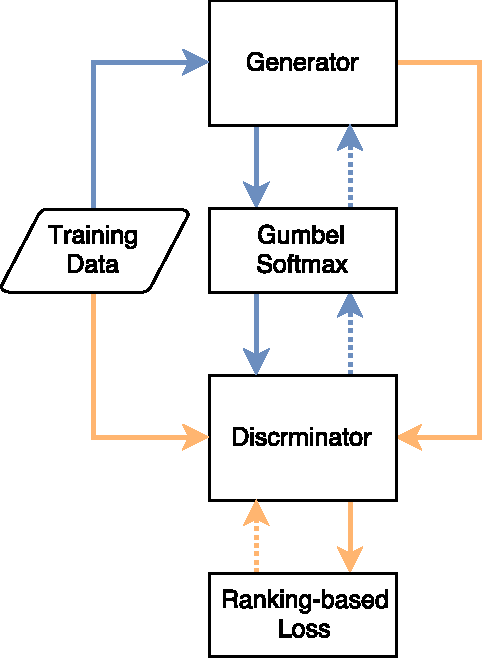
\includegraphics[width=0.35\textwidth]{images/overview.pdf}
    \caption{Overview of our adversarial training setting. The solid lines indicate the flow of training data and dash lines show the back propagation direction of gradients. Orange lines illustrate the process in which the discrminator uses generated negative samples and maximize the ranking-based objective. Blue lines shows the generator use discrminator as its feedback and propagate the gradient through gumbel softmax~\cite{GumbelSoftmax_Jiang_2016}.}
\label{system-overview}
\end{figure}


\subsection{Generator}

The generator will output an probabilistic measure of the set of all entities $\mathcal{E}$. We minimize the following cross entropy term defined through the discrminators' feedback,

\begin{align*}
    \min_g \sum_{(h, r, t)\in X}
        \mathbb{E}_{\tilde t \sim p_g(t \mid h, r)}
            \frac{\exp(d(h, r, \tilde t) / \tau)}
                 {\sum_{t^* \in \{ t, \tilde t\}} \exp(d(h, r, t^*) / \tau)}
\end{align*}

However, it's not possible to directly optimize the above loss function using gradient-based algorithms. In practice, we have to sample a discrete distribution, which makes a simple reparemeterization trick~\cite{VAE} fail. A popular solution to this problem is to adopt reinforcement learning. The REINFORCE algorithm~\cite{Williams_1992}, for example, reformulates the gradient of the generator objective above but is known to be hard to train and meets the problem of cold start. Furthermore, the gradients it produced tend to have high variance, though a baseline term was added in our experiments.

Since the generator actually gives a multinomial distribution, we adopt the gumbel softmax~\cite{GumbelSoftmax_Jiang_2016} which uses gumbel noise to reparemeterize the multinomial distribution. Specifically, we add standard gumbel noise to the unnormalized log probabilities (logits) and do softmax as follows,
\begin{align*}
    GumbelProb_i = \frac{\exp((logits_i + z_i)/ \tau)}{\sum_{j}\exp((logits_j + z_j)/ \tau)},
\end{align*}
where $z \sim Gumbel(0, 1)$ is the sampled gumbel noise, $logits$ is the output of the generator, and $\tau$ is the positive temperature. As $\tau$ descreases towards 0, the gumbel probability will approximate a one-hot vector sampled from the categorical distribution parameterized by the output logits, which differs from the original gumbel max trick that it is differentiable w.r.t.\ the $logits$. Blue lines in Figure~\ref{system-overview} illustrate the generator learning process, too.


\subsection{Pretraining and ensemble}

\paragraph{Pretraining} As GANs are hard to train, we introduce a pretraining procedure at first. Note the setting in previous subsections only works when the generator and discrminator are trained adversarially and alternatively. When it comes to the pretraining, we have to design new loss functions for them separately.

To keep things simple, we minimize the cross entropy loss for the generator as below,
\[
    \min_g -\sum_{(h, r, t)\in X} p_g(t \mid h, r),
\]

For the discrmininator, we either use the similar hinge loss with margin as TransE~\cite{TransE2013},
\[
    \min_d \sum_{\substack{(h, r, t)\in S,\\ (h^\prime, r, t^\prime)\in S^\prime }}
        {[ d(h, r, t) - d(h^\prime, r, t^\prime) + \gamma ]}_+,
\]
where ${[\cdot]}_+$ denote the hinge loss, $\gamma$ is the margin hyperparameter. $S$ may either denotes the positive or negative samples. If we want the discriminator to give smaller scores for better samples, $S$ is the set of positive samples and $S'$ the set of negative ones, and vice vesa.

\paragraph{Ensemble} Construction of ensemble among base learners is beneficial to performance improvements~\cite{dietterich2000ensemble}. Because of the adversarial training setting, the discrmininator and generator are two heterogeneous models and suitable for ensemble learning. We construct a simple weighted average method to exploits both models,
\[
    s(h, r, t) = \alpha d(h, r, t) + (1 - \alpha) p_g(t \mid h, r),
\]
where $\alpha$ is a hyperparameter tuned on the validation set.

% --------------------------------------
% related work

\section{Related work}

We continue to discuss the work related to ours and make comparisons with them in this section.

\paragraph{Translation models} As discussed in Section~\ref{sec:intro}, TransE~\cite{TransE2013} is a representative model adopting the translation assumption. Specifically, they try to minimize the following hinge loss,
\[
    \min\sum_{\substack{(h, r, t)\in S,\\ (h^\prime, r, t^\prime)\in S^\prime }}
        {\left[\gamma + f(h, r, t) - f(h^\prime, r, t^\prime)\right]}_+,
\]
where $S$ is the set of triples and $S'$ is the set of negative samples. $f(h, r, t)$ can be viewed as an energy or scoring function which in their case is an L1 or L2 norm of $h + r - t$. TransH~\cite{TransH2014} extends the basic TransE by projecting entities to the hyperplaned defined by the relation. Let $\omega_r$ be the normal vector of the hyperplane, then the scoring function in TransH is defined as $f(h, r, t) = \lVert(h~-~\omega_r^T h \omega_r) + d_r -~(t~-~\omega_r^T t \omega_r)\rVert_2^2 $.
TransR~\cite{TransR2015} futher extends the idea by making the relation a complete space rather than a hyperplane in entity space. With a linear mapping between these two spaces, their scoring function is $f(h, r, t) = \lVert hM_r + r - h M_r \rVert_2^2$. These models differ from ours both in its discrmininative nature and the translation assumption.

TransG~\cite{TransG} is a generative model and is thus closest to our work. It draws head and tail entities from gaussian distributions, and draw the relation from a mixture of both entities. It uses the Chinese restaurant process to model the relation token implying different semantics, namely the \emph{multi-semantic phenomenon}.
On the contrary, our model doesn't assume explicit gaussian density, but uses the adversarial framework to approximate the unknown real data distribution, which is a merit of GAN~\cite{Goodfellow_2016}.

\paragraph{Neural models} Apart from the translation-based scoring function, Structured Embedding~\cite{bordes2011structured_embedding} is the start of the other approach, which defines the scoring functions using two matrices as $f(h, r, t) = \lVert M_{r,1}h - M_{r,2}t \rVert_{L1}$. Latent Factor Model~\cite{jenatton2012bilinear} uses a bilinear model to characterize the relation between two entities with the scoring function as $f(h, r, t) = h^T W_r t$.
Single Layer Model is a baseline in Socher et al.~\cite{NTN}, which use one single layer neural network as the scoring function, namely $f(h, r, t)=u_r^T \tanh(W_r[h;t])$. They further propose the most expressive Neural Tensor Network (NTN) model, which utilizes the merits of both the bilinear model and single layer neural network. The scoring function is $u_r^T \tanh(h^T W_r^{[1:k]}t + V_r[h;t] + b_r)$. Due to the large amount of parameters, it's not easy to train NTN on large scale data.

\paragraph{GANs} Then let's move on to the GANs. GAN~\cite{GAN} proposes a vivid explaination of the minimax game between a discriminator and a generator, which sheds the light on the image processing field~\cite{Ledig_2017_CVPR}. However, classic GAN is hard to train~\cite{Salimans_2016}. Through a detailed analysis on the objective, Arjovsky et al.\ proposed Wasserstein GAN~\cite{Arjovsky2017WGAN} which replaces the Jensen-Shannon divergence with the Earth-Mover distance. They also reported new techniques for training~\cite{Gulrajani2017LipschitzReg}, which aims to add penalty into gradients to enforce the Lipschitz constraint.

In the field of natural language processing, SeqGAN~\cite{SeqGAN} is proposed to generate natural language sentences. They also use policy gradient method to backpropagate through discrete sampling. To evaluate the reward of generated sentences in advance, they use Monte Carlo tree search to roll out the whole sentence and use the samples' reward to update in the middle of generation. RankGAN~\cite{RankGAN} futher extends the idea by incorporating the ranking-based loss, which tries to optimize the list-wise ranking of the generated sentence in a candidate list. The recently proposed IRGAN~\cite{IRGAN} nevertheless brings the adversarial training idea into the Information Retrieve field, which unifies both the discriminative and generation schools in a single framework. These models inspired us to use ranking as objective and to combine two models.

Tramèr et al.~\cite{EnsembleAdvTraining} recently proposed a novel framework called Ensemble Adversarial Training. Along with the progress in using adversarial examples to attack trained models, they propose an extension of GAN that augments training data with perturbation using pretrained models, which is reminiscent of boosting methods in ensemble learning, and differs from our method that adopts the weighted average idea between the heterogeneously trained generator and discrmininator.


% --------------------------------------
% experiments

\section{Experiments}

% --------------------------------------
% conclusion

\section{Conclusion}

% --------------------------------------
\section*{References}

\bibliography{adv-kb2e-bibfile}

\end{document}

% ====================================================
% reference snippets

% \paragraph{Installation} If the document class \emph{elsarticle} is not available on your computer, you can download and install the system package \emph{texlive-publishers} (Linux) or install the \LaTeX\ package \emph{elsarticle} using the package manager of your \TeX\ installation, which is typically \TeX\ Live or Mik\TeX.

% \paragraph{Usage} Once the package is properly installed, you can use the document class \emph{elsarticle} to create a manuscript. Please make sure that your manuscript follows the guidelines in the Guide for Authors of the relevant journal. It is not necessary to typeset your manuscript in exactly the same way as an article, unless you are submitting to a camera-ready copy (CRC) journal.

% \paragraph{Functionality} The Elsevier article class is based on the standard article class and supports almost all of the functionality of that class. In addition, it features commands and options to format the
% \begin{itemize}
% \item document style
% \item baselineskip
% \item front matter
% \item keywords and MSC codes
% \item theorems, definitions and proofs
% \item lables of enumerations
% \item citation style and labeling.
% \end{itemize}

% The author names and affiliations could be formatted in two ways:
% \begin{enumerate}[(1)]
% \item Group the authors per affiliation.
% \item Use footnotes to indicate the affiliations.
% \end{enumerate}
% See the front matter of this document for examples. You are recommended to conform your choice to the journal you are submitting to.